\section{Dummy signal testing of the regular and variational Autoencoder}

Another important part of benchmarking the algorithm is to test it on a signal sample. This is the closest test we can do before
we no longer can alter the algorithm, as that would be supervised learning. Results from both the regular and the variational autoencoder 
are shown below. 

\subsection*{Autoencoder}

\begin{figure}[h!]
    \centering
    \begin{subfigure}{.45\textwidth}
        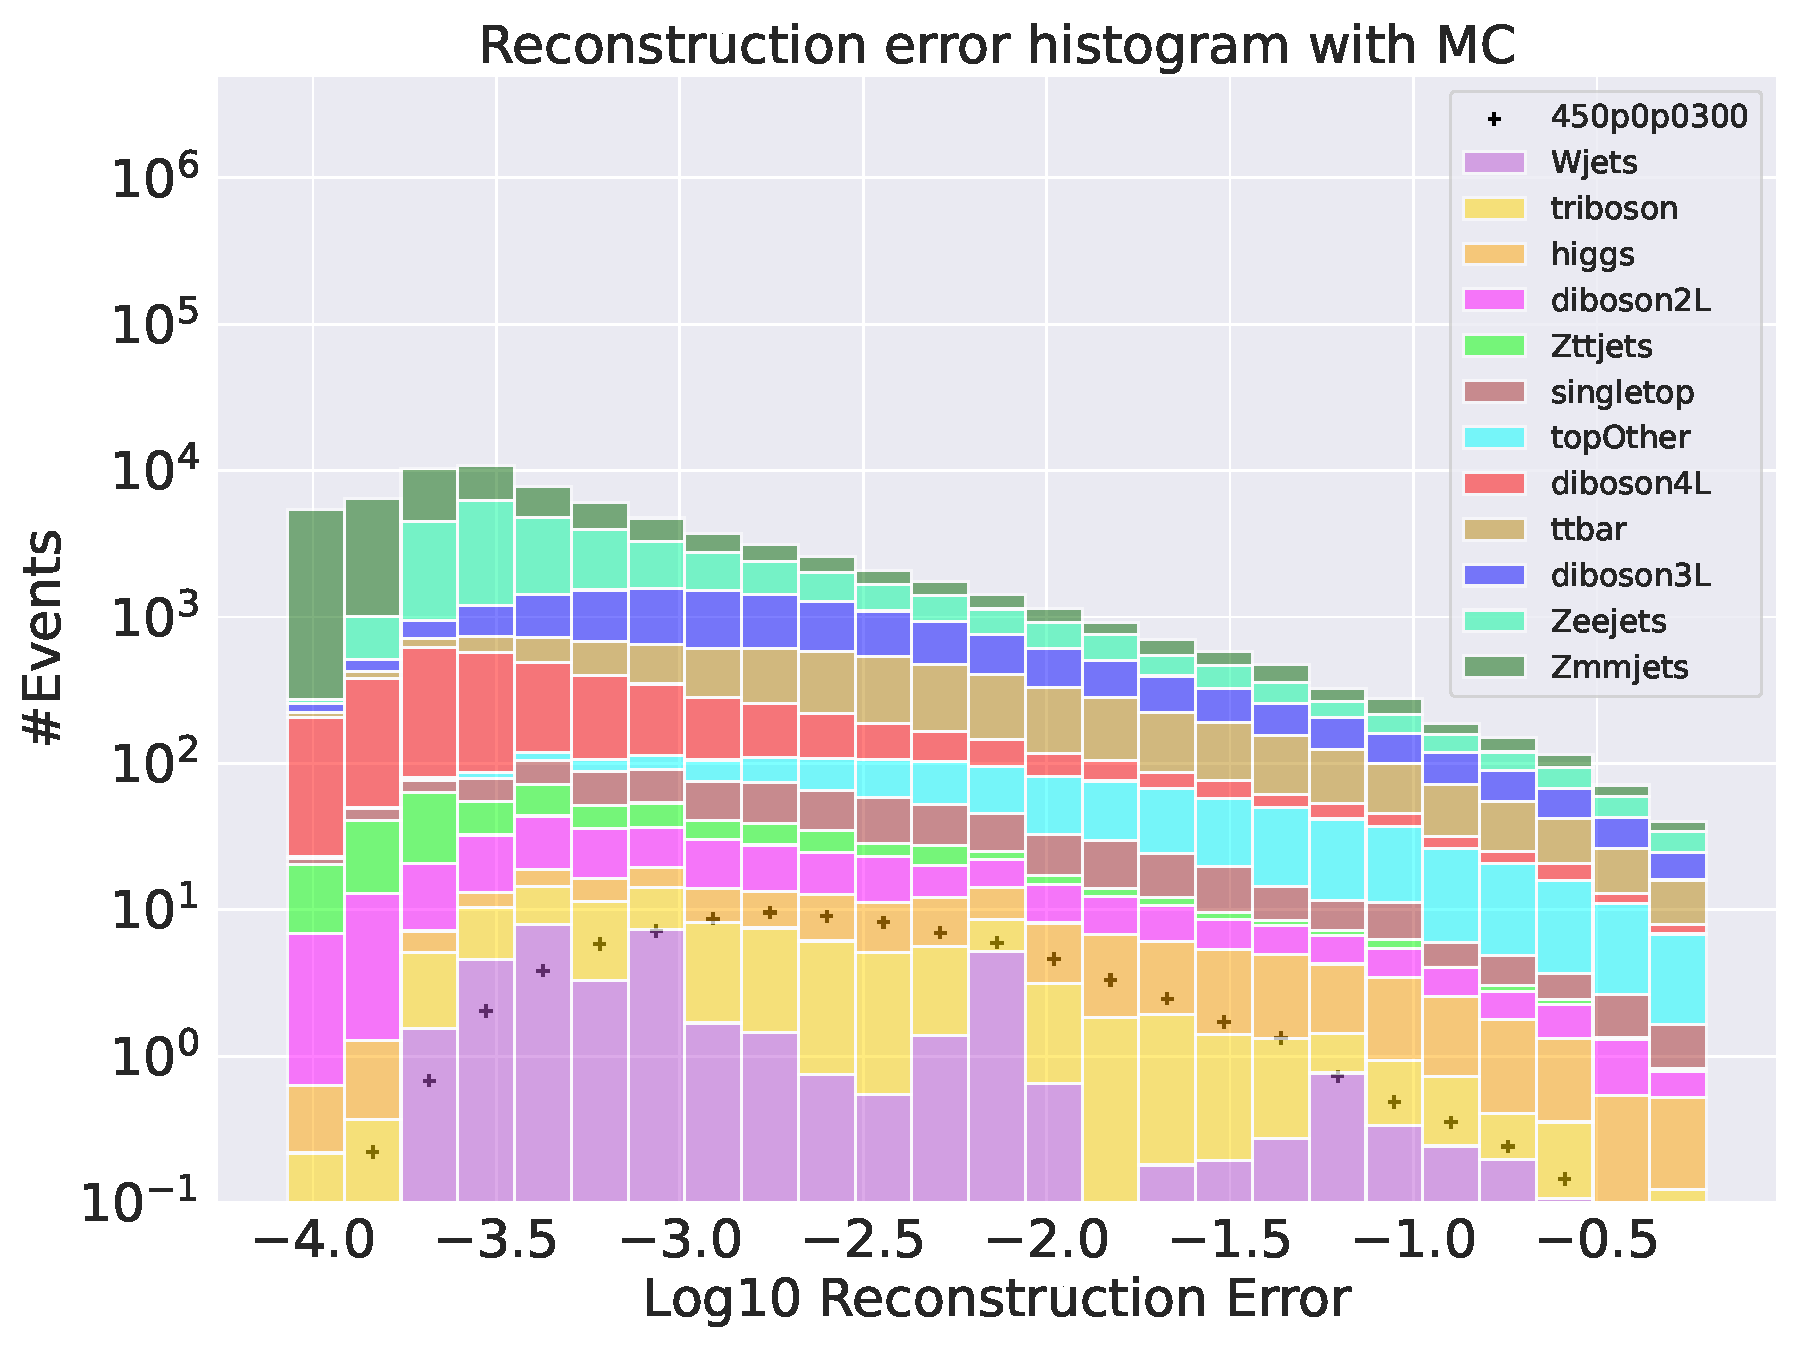
\includegraphics[width=\textwidth]{Figures/AE_testing/small/b_data_recon_big_rm3_feats_sig_450p0p0300.pdf}
        \caption{Reconstruction error on validation SM MC from the Autoencoder. The susy signal is the $450-300$ sample. 
        No significant separation of the distributions are found. }
        \label{fig:ae_susy_450_300_recon}
    \end{subfigure}
    \hfill
    \begin{subfigure}{.45\textwidth}
        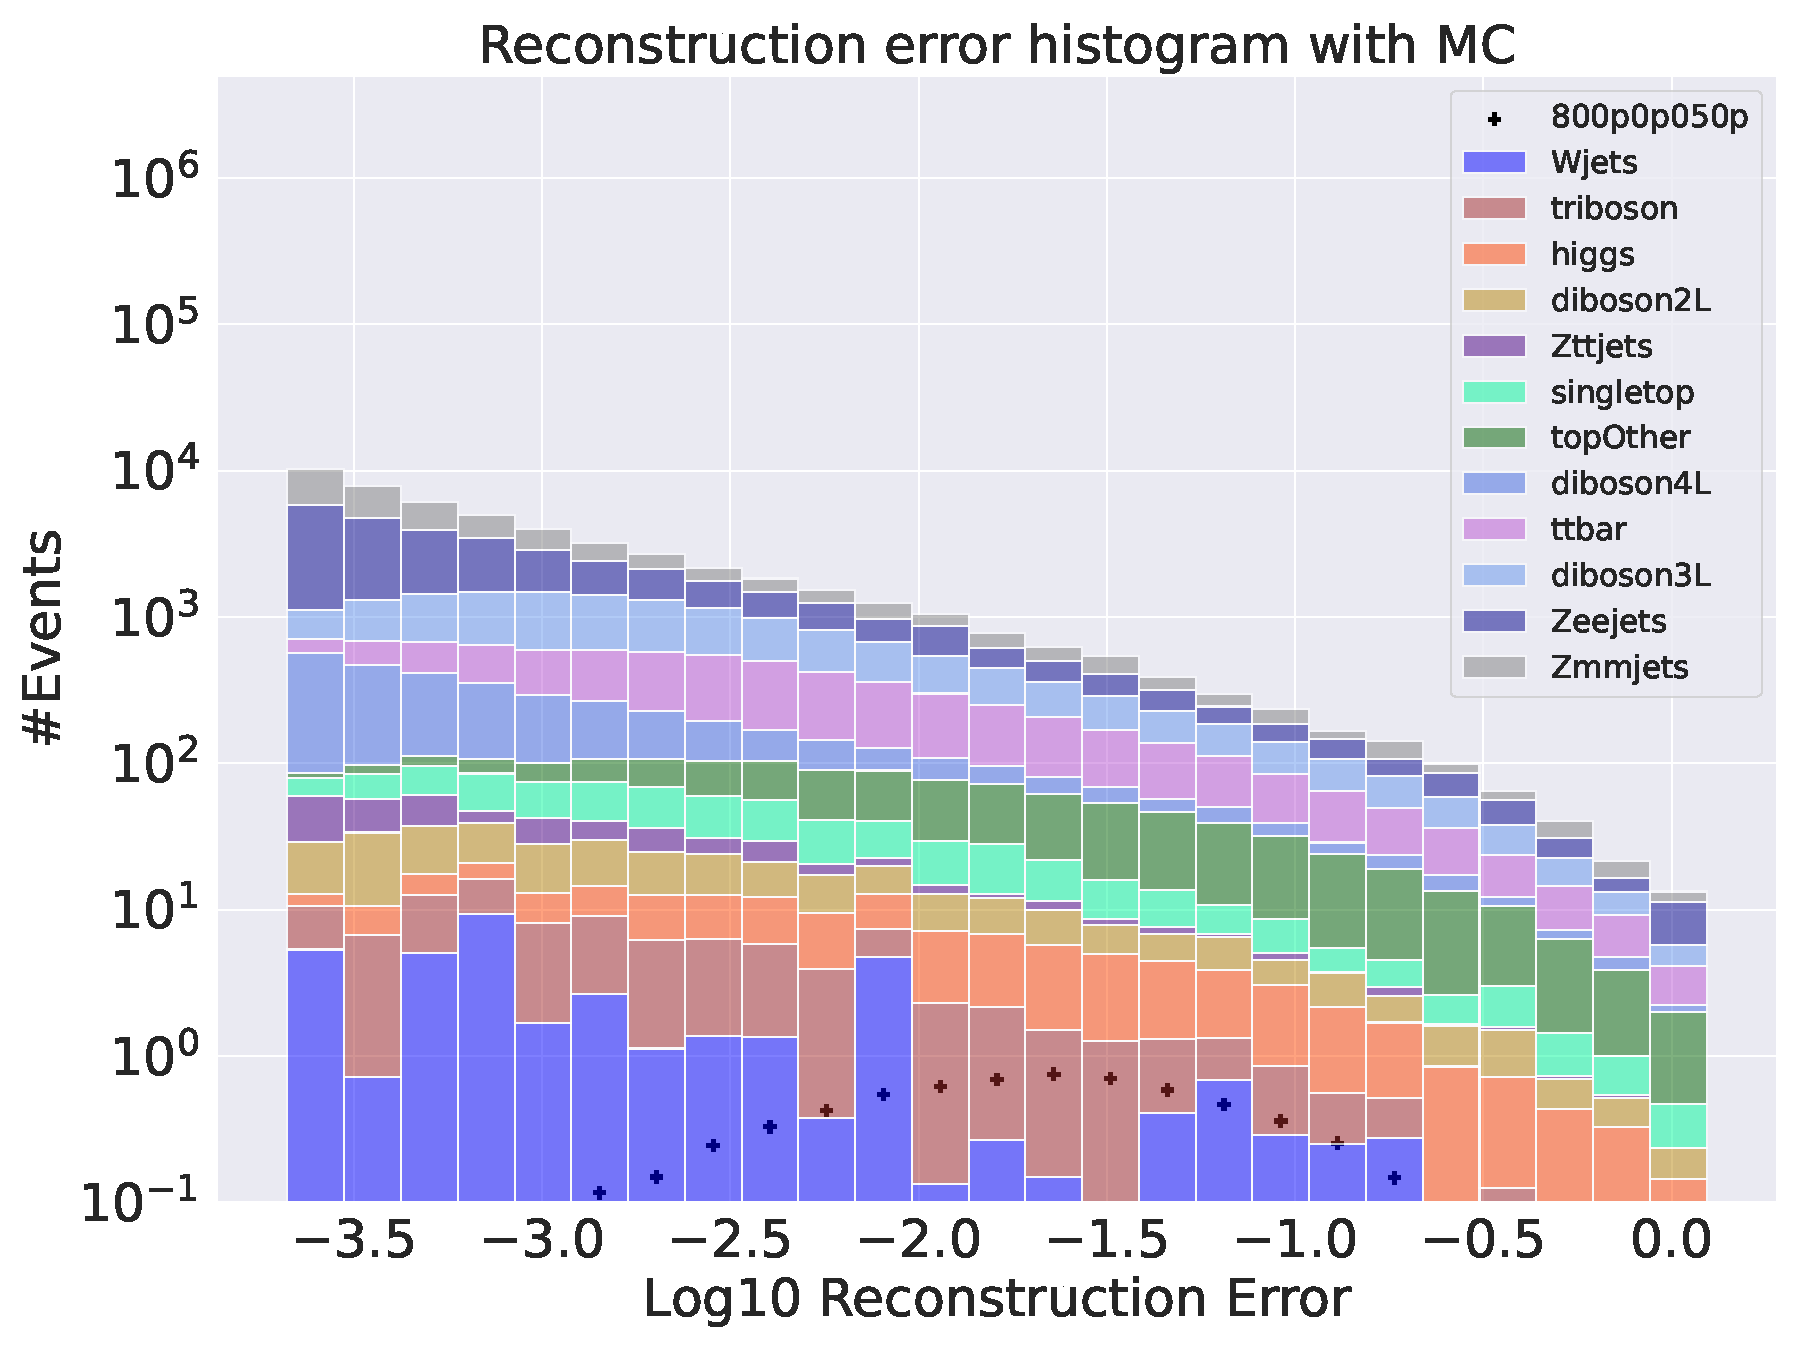
\includegraphics[width=\textwidth]{Figures/AE_testing/small/b_data_recon_big_rm3_feats_sig_800p0p050p.pdf}
        \caption{Reconstruction error on validation SM MC from the Autoencoder. The susy signal is the $800-50$ sample. 
        No significant separation of the distributions are found. }
        \label{fig:ae_susy_800_50_recon}
    \end{subfigure}
    \hfill
    \begin{subfigure}{.45\textwidth}
        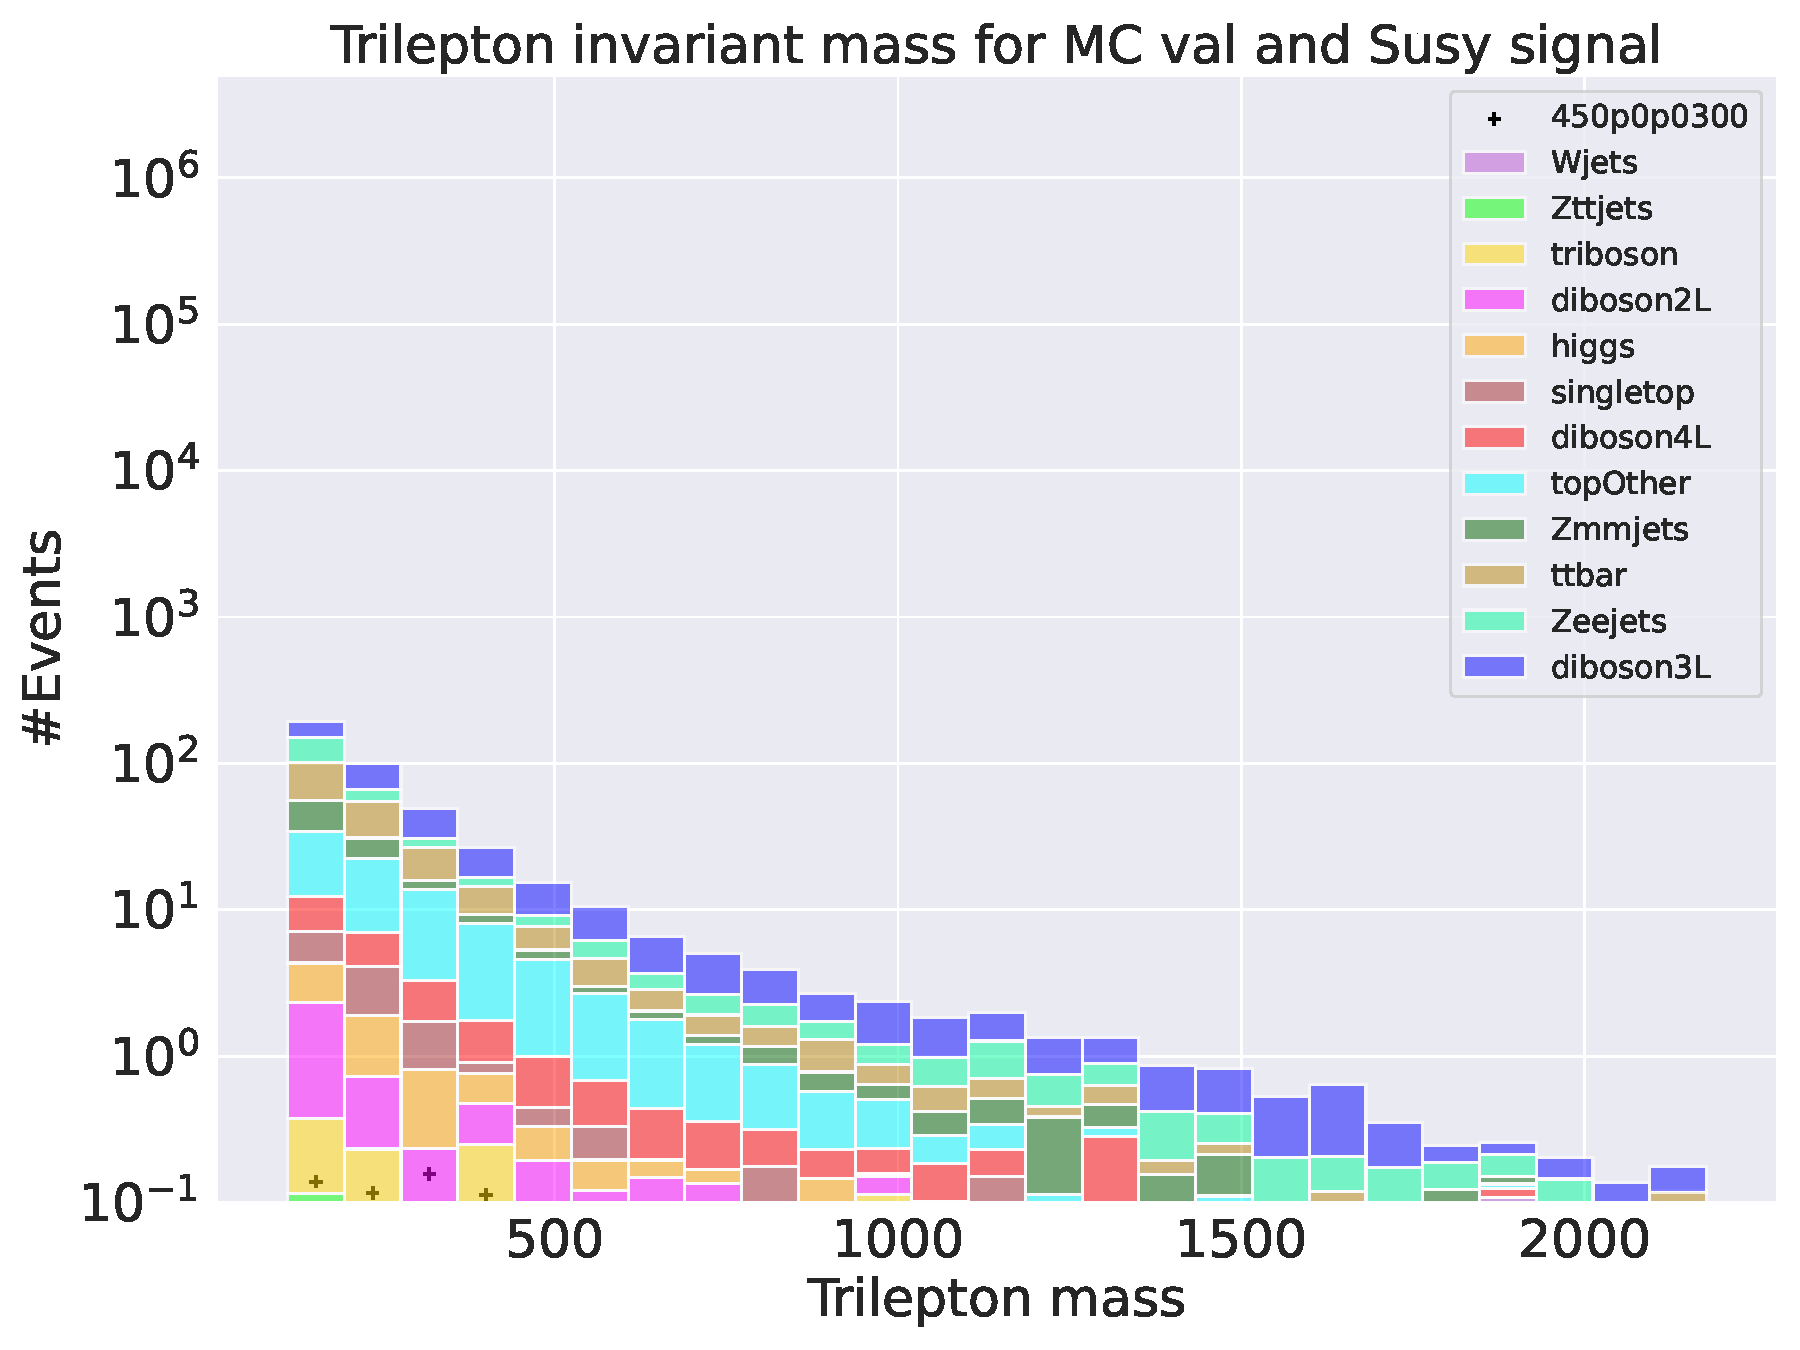
\includegraphics[width=\textwidth]{Figures/AE_testing/small/b_data_recon_big_rm3_feats_sig_450p0p0300_Trilepton mass.pdf}
        \caption{Trilepton mass bump search for the $450-300$ susy signal. Here events are selected only if reconstruction error is larger than 1. No significant 
        separation of distribution found.}
        \label{fig:ae_susy_450_300_trilep}
    \end{subfigure}
    \hfill        
    \begin{subfigure}{.45\textwidth}
        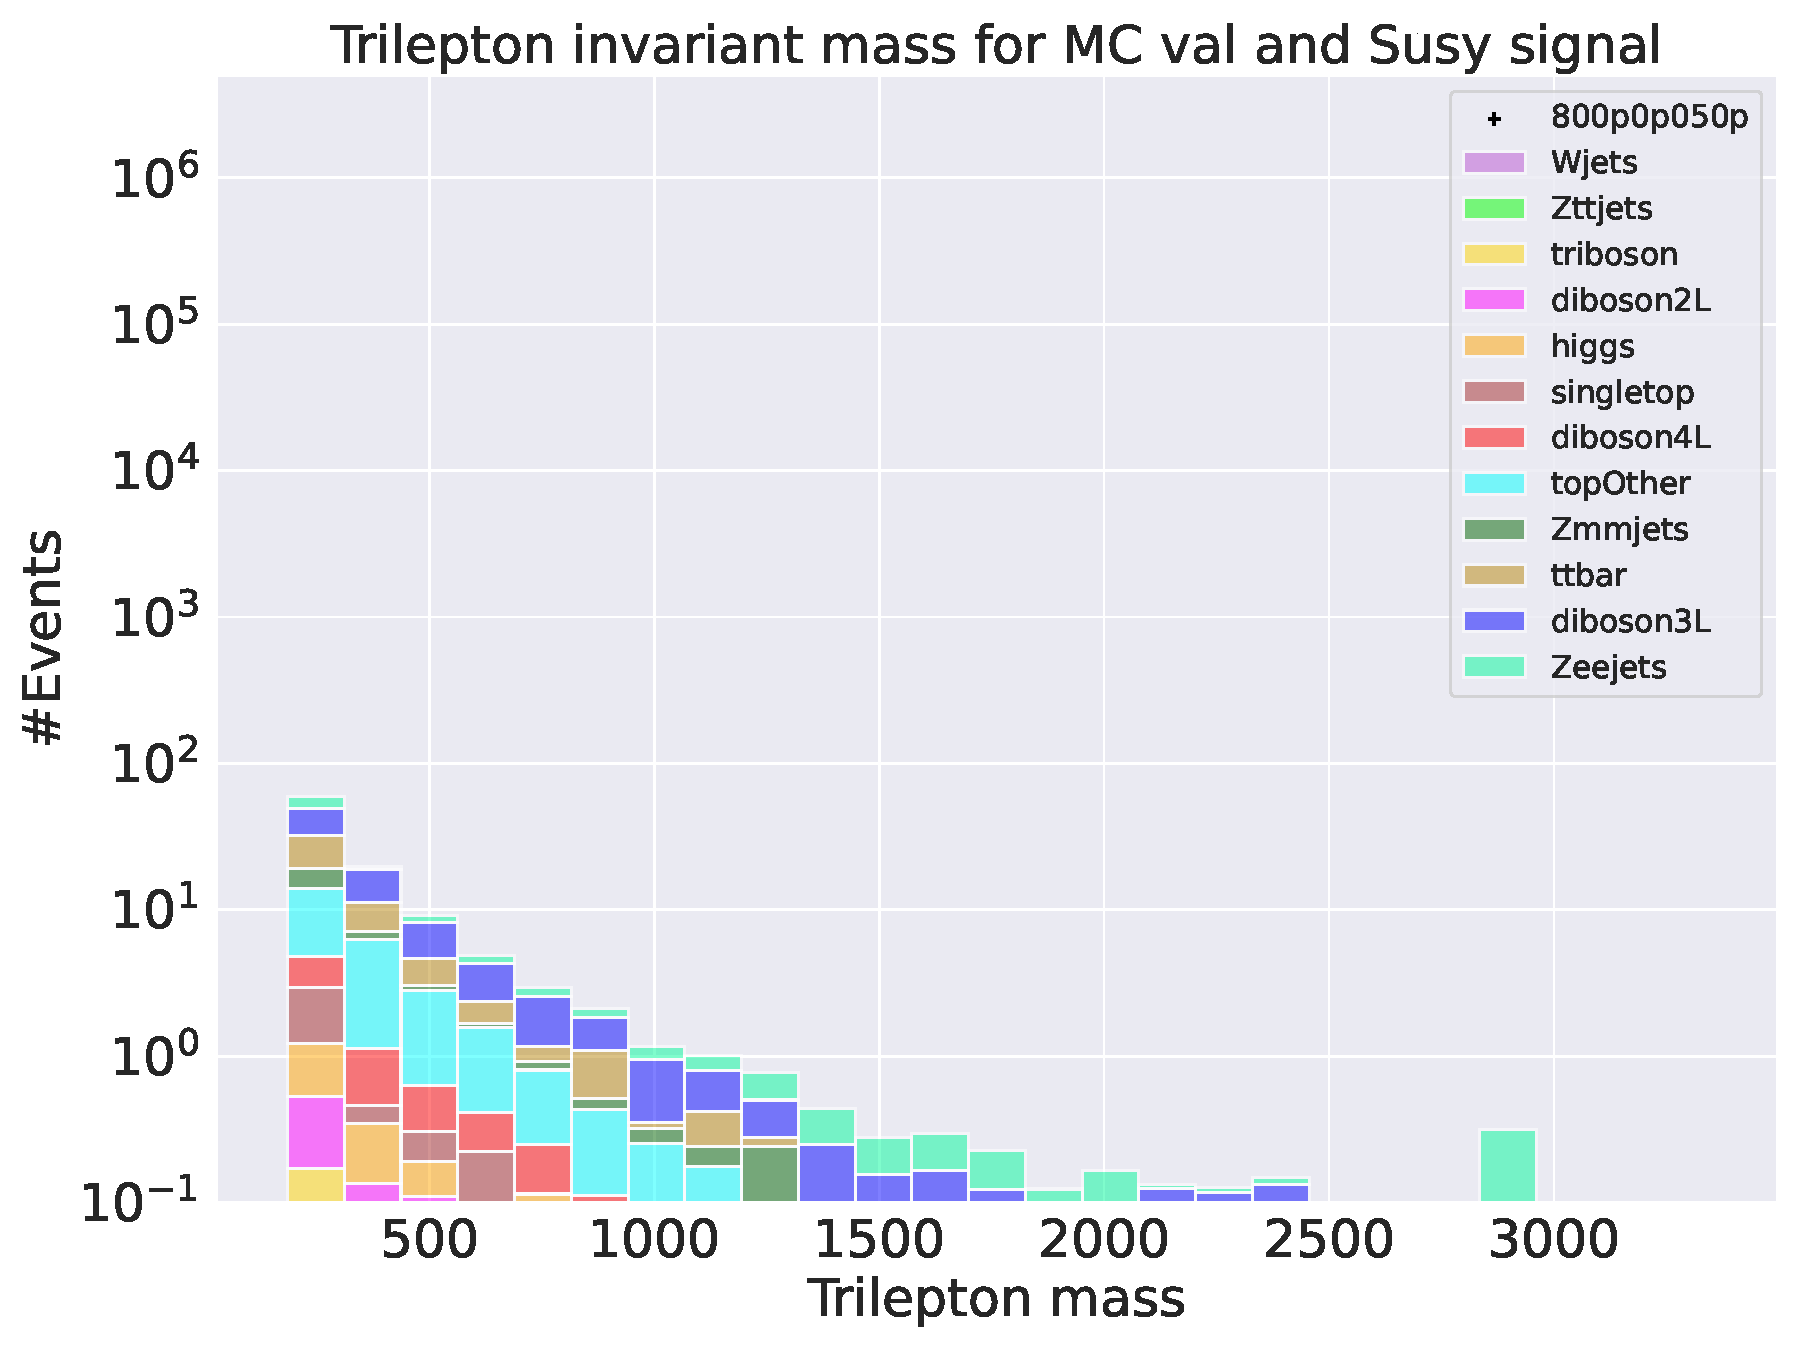
\includegraphics[width=\textwidth]{Figures/AE_testing/small/b_data_recon_big_rm3_feats_sig_800p0p050p_Trilepton mass.pdf}
        \caption{Trilepton mass bump search for the $800-50$ susy signal. Here events are selected only if reconstruction error is larger than 1. No significant 
        separation of distribution found.}
        \label{fig:ae_susy_800_50_trilep}
    \end{subfigure} 
    \hfill     
    \caption{Reconstruction error and trilepton mass bump search on the $450-300$ and $800-50$ susy signals. The reconstruction error cut is set to 1. }
    \label{fig:ae_susy_450_300_800_50_recon_trilep}
\end{figure}


\subsection*{Variational Autoencoder}

\begin{figure}[h!]
    \centering
    \begin{subfigure}{.45\textwidth}
        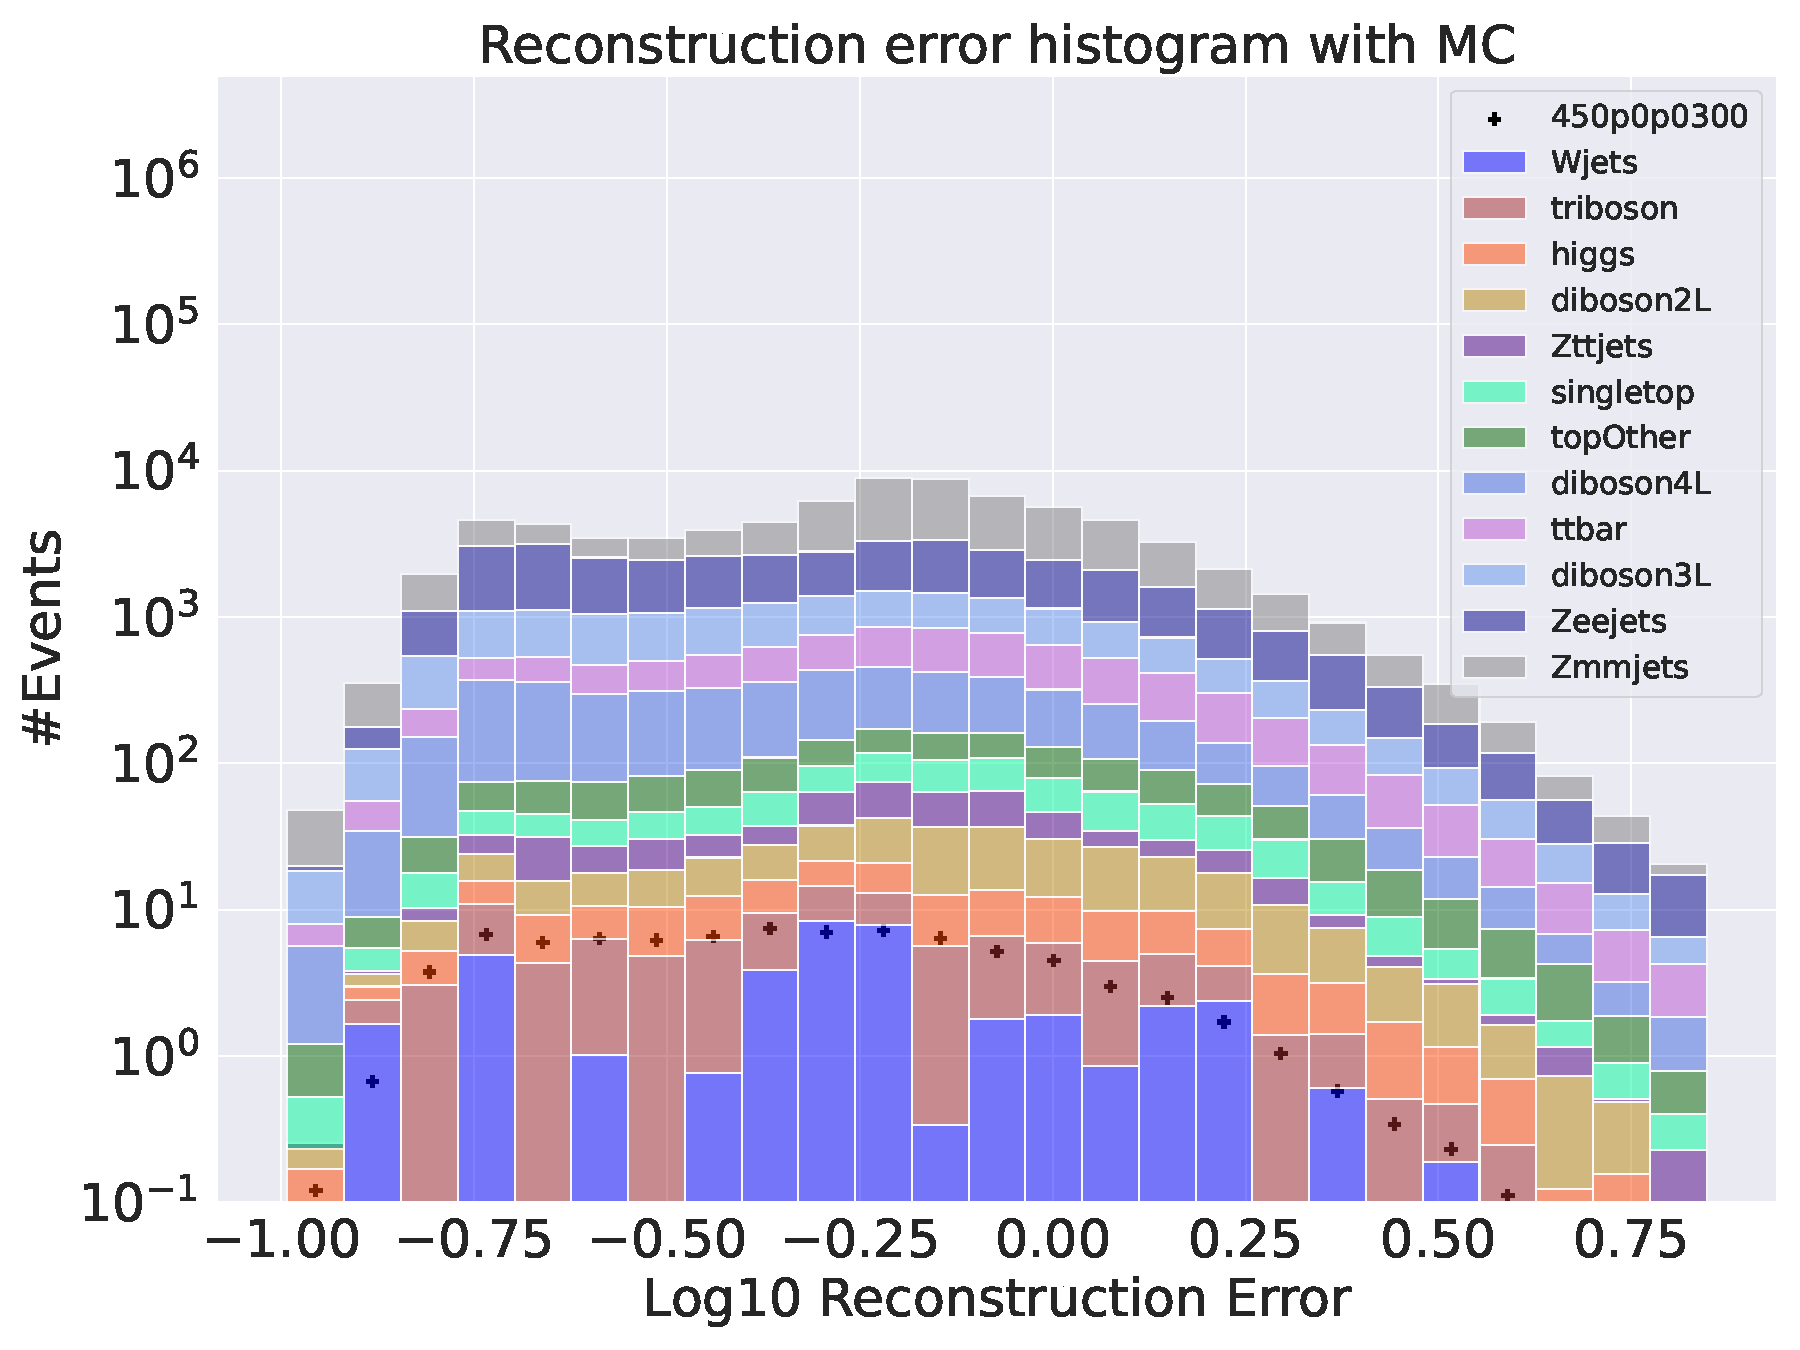
\includegraphics[width=\textwidth]{Figures/VAE_testing/small/b_data_recon_big_rm3_feats_sig_450p0p0300.pdf}
        \caption{Reconstruction error on validation SM MC from the variational Autoencoder. The susy signal is the $450-300$ sample. 
        No significant separation of the distributions are found. }
        \label{fig:vae_susy_450_300_recon}
    \end{subfigure}
    \hfill
    \begin{subfigure}{.45\textwidth}
        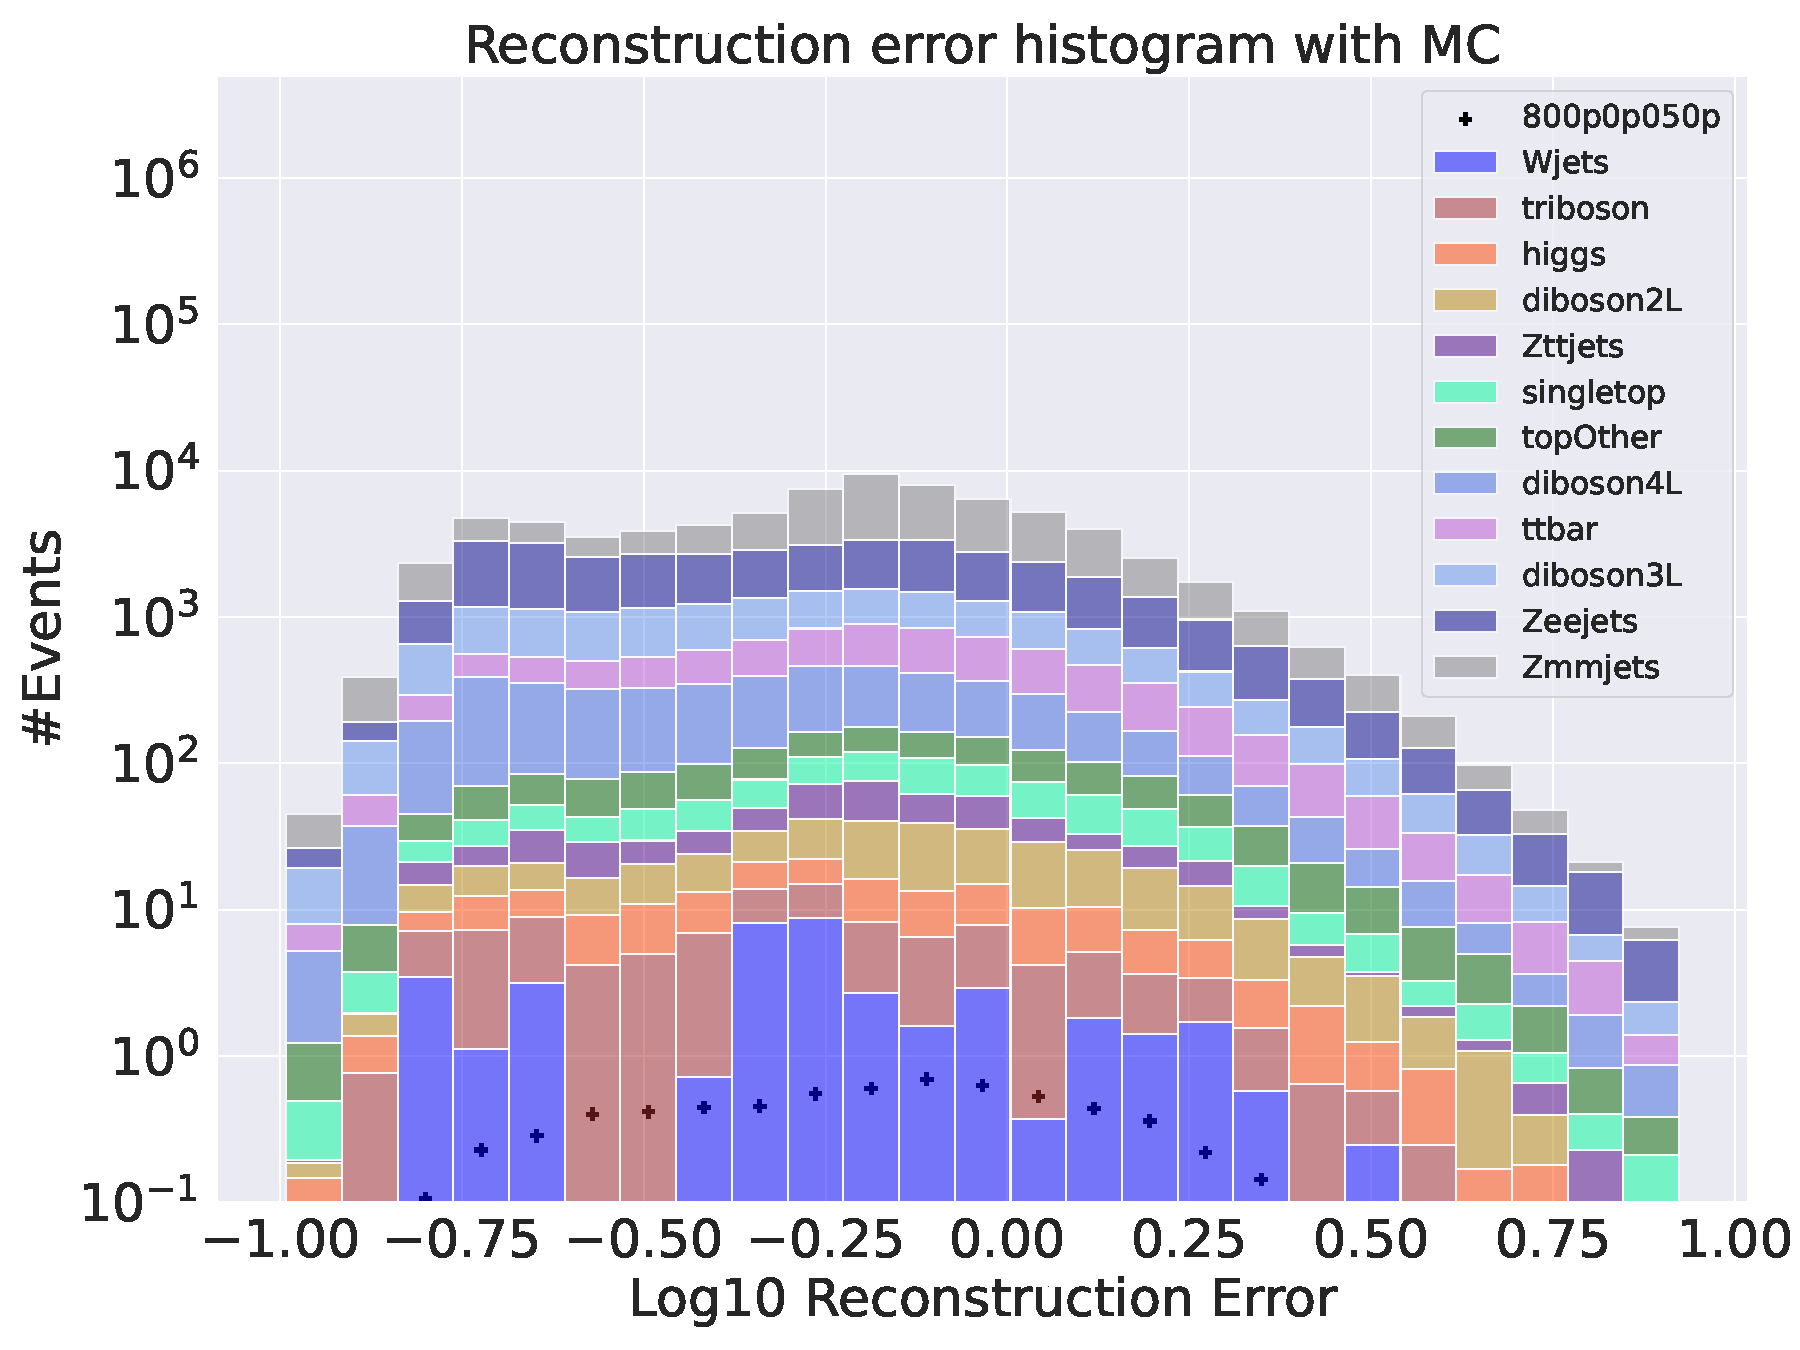
\includegraphics[width=\textwidth]{Figures/VAE_testing/small/b_data_recon_big_rm3_feats_sig_800p0p050p.pdf}
        \caption{Reconstruction error on validation SM MC from the variational Autoencoder. The susy signal is the $800-50$ sample. 
        No significant separation of the distributions are found. }
        \label{fig:vae_susy_800_50_recon}
    \end{subfigure}
    \hfill
    \begin{subfigure}{.45\textwidth}
        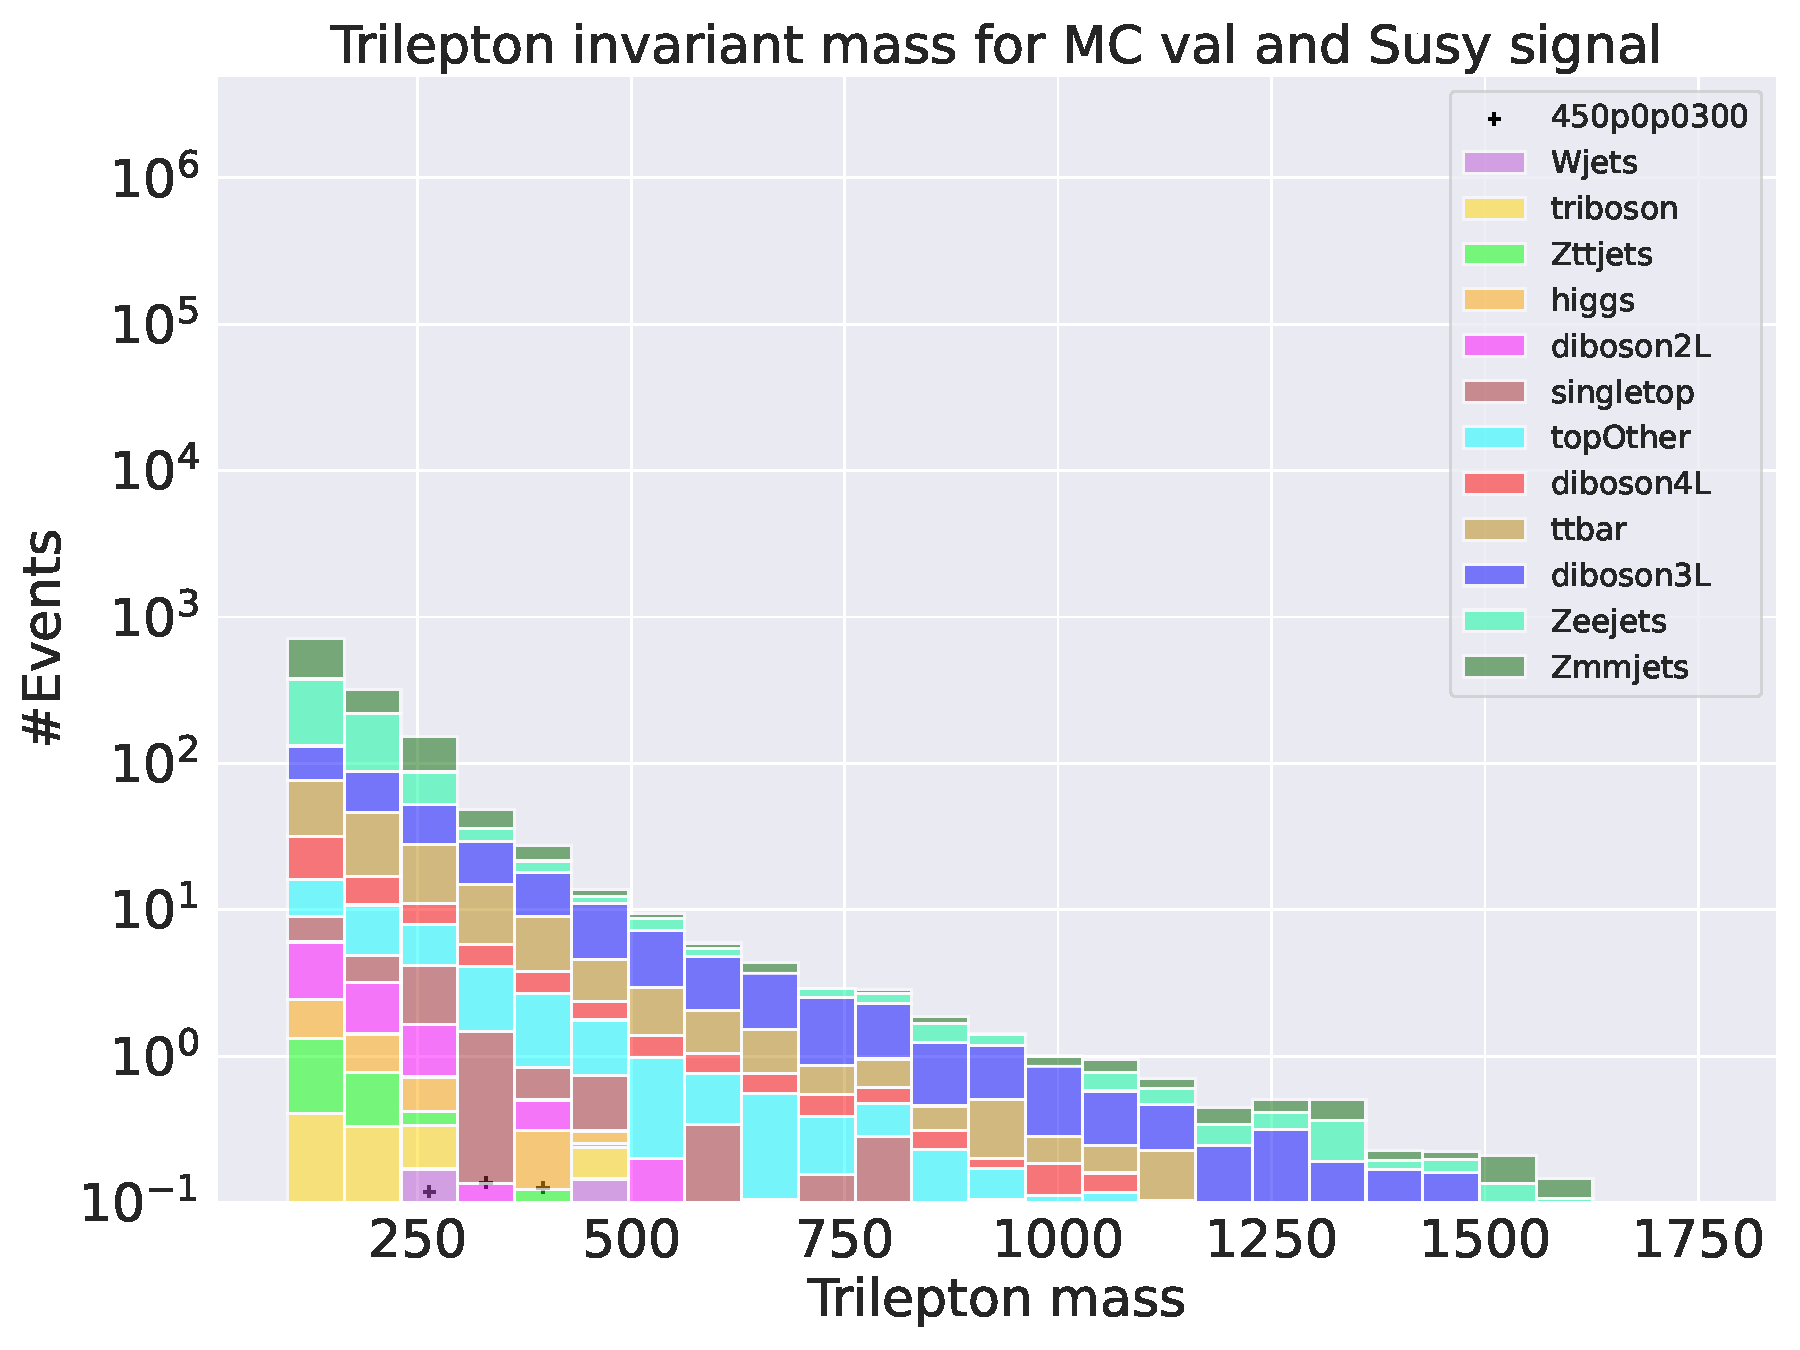
\includegraphics[width=\textwidth]{Figures/VAE_testing/small/b_data_recon_big_rm3_feats_sig_450p0p0300_Trilepton mass.pdf}
        \caption{Trilepton mass bump search for the $450-300$ susy signal. Here events are selected only if reconstruction error is larger than 1. No significant 
        separation of distribution found.}
        \label{fig:vae_susy_450_300_trilep}
    \end{subfigure}
    \hfill   
    \begin{subfigure}{.45\textwidth}
        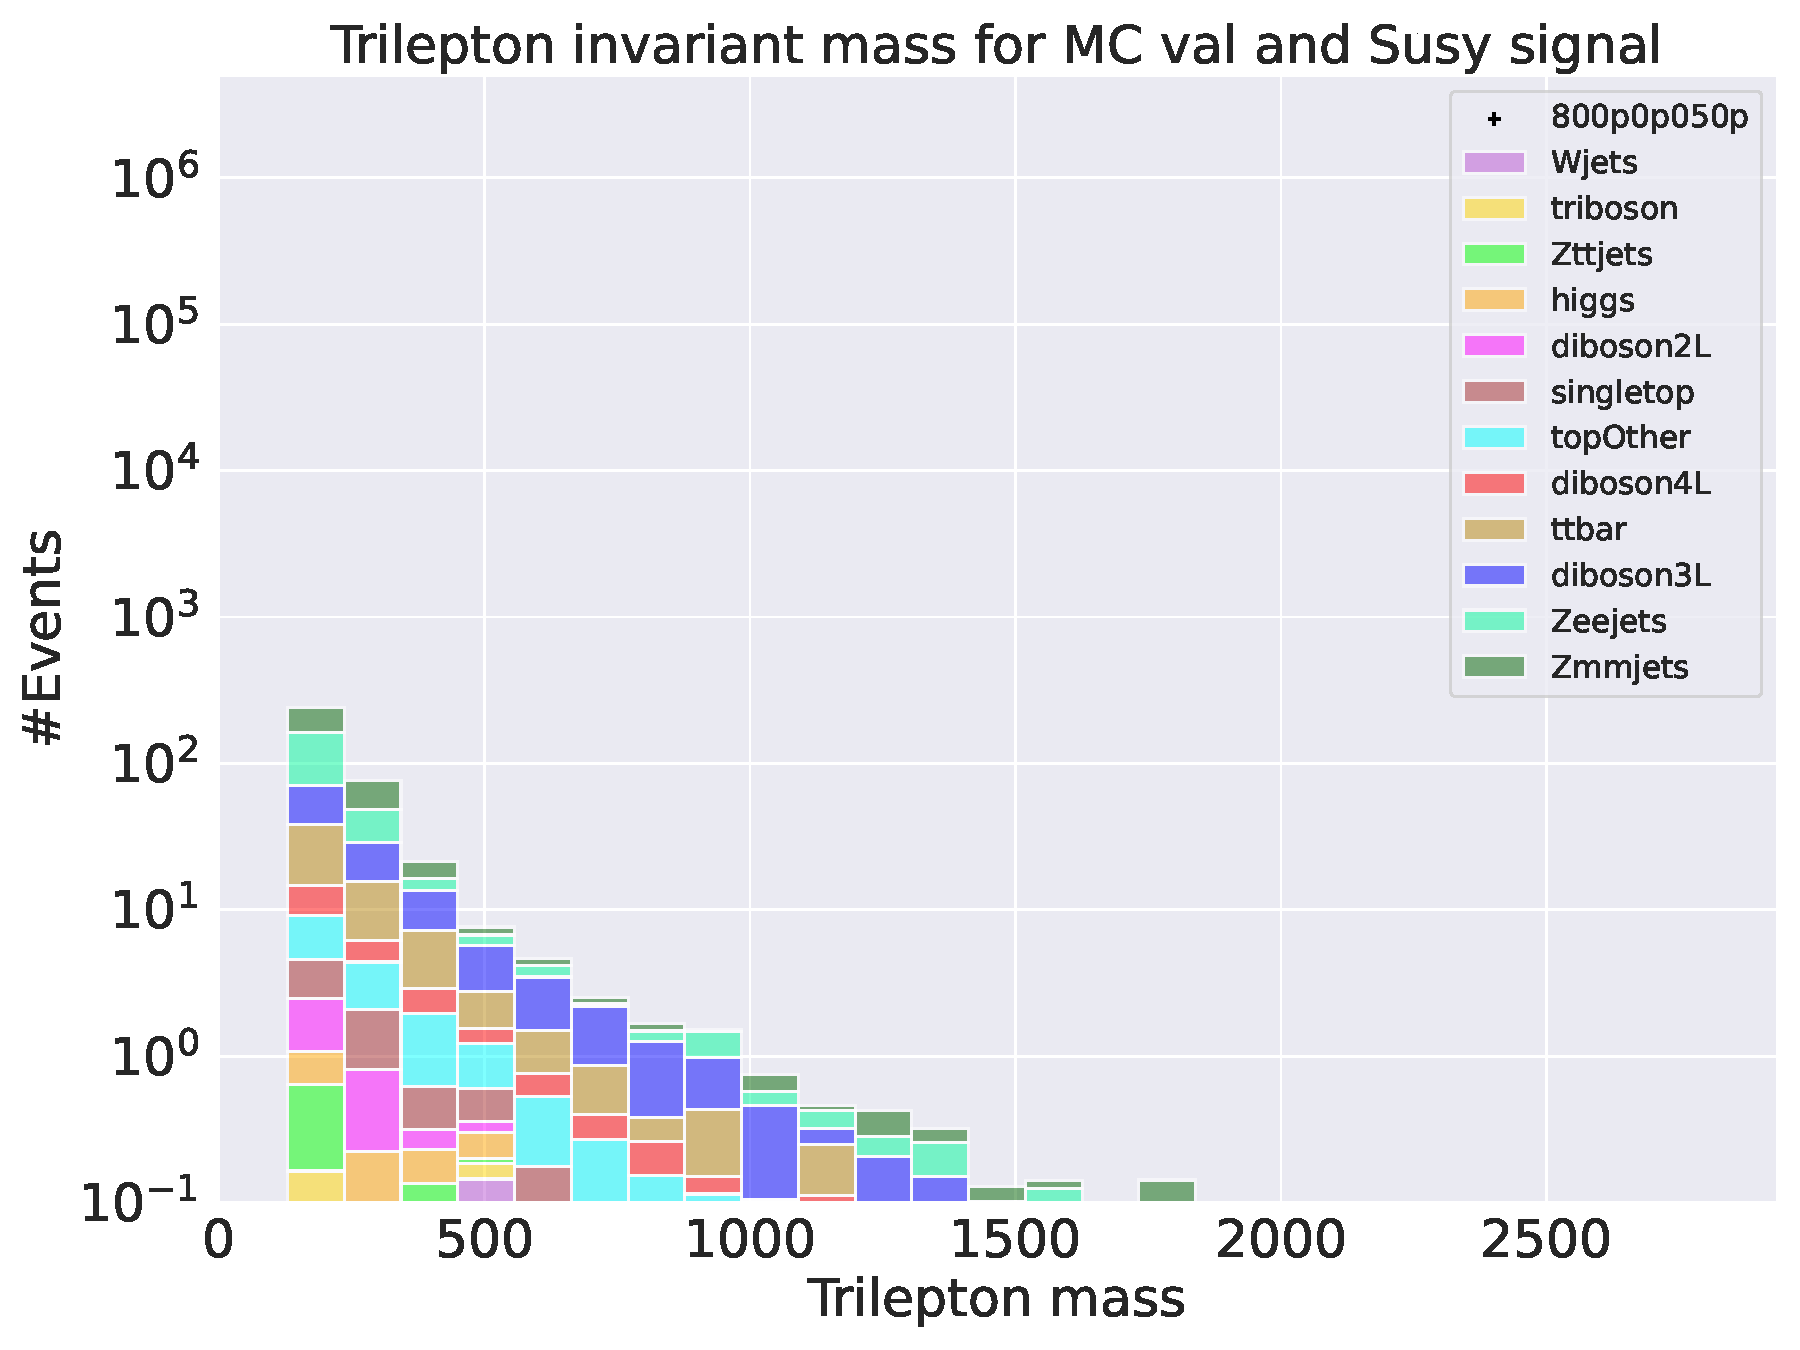
\includegraphics[width=\textwidth]{Figures/VAE_testing/small/b_data_recon_big_rm3_feats_sig_800p0p050p_Trilepton mass.pdf}
        \caption{Trilepton mass bump search for the $800-50$ susy signal. Here events are selected only if reconstruction error is larger than 1. No significant 
        separation of distribution found.}
        \label{fig:vae_susy_800_50_trilep}
    \end{subfigure}
    \hfill      
    \caption{ Reconstruction error and trilepton mass bump search on the $450-300$ and $800-50$ susy signals. The reconstruction error cut is set to 1.}
    \label{fig:vae_susy_450_300_800_50_recon_trilep}
\end{figure}


\newpage